\documentclass[11pt]{article}
\usepackage{graphicx}
% Default margins are too wide all the way around. I reset them here
\setlength{\topmargin}{-.5in}
\setlength{\textheight}{9in}
\setlength{\oddsidemargin}{.125in}
\setlength{\textwidth}{6.25in}
\begin{document}
\title{Finite State Machine Grammar for MiPal}
\author{Vlad Estivill-Castro\\Ren\'{e} Hexel\\
{\tt www.mipal.net.au }
}
%\renewcommand{\today}{November 2, 1994}
\maketitle
\section {The Finite State Machines in MiPal}
These are described in three parts.
\begin{enumerate}
\item A transitions file providing the transition table, this file
must start with {\tt T} and has extension {\tt .txt}.
\item A actions file providing what happens one each state,
this file must start with {\tt A} and has extension {\tt .txt}.
\item Files that describe the inference to make conclusion
about the predicates that label the transitions. Usually
should end with extension {\tt d}. They re currently CDL
files, but expect to improve to also Prolog soon.
\end{enumerate}
\subsection{About the implementation}
Using doxygen, documentation is available for the implementation. The following diagrams
are taken from the generated documentation to illustrate the structure further.
\begin{figure}
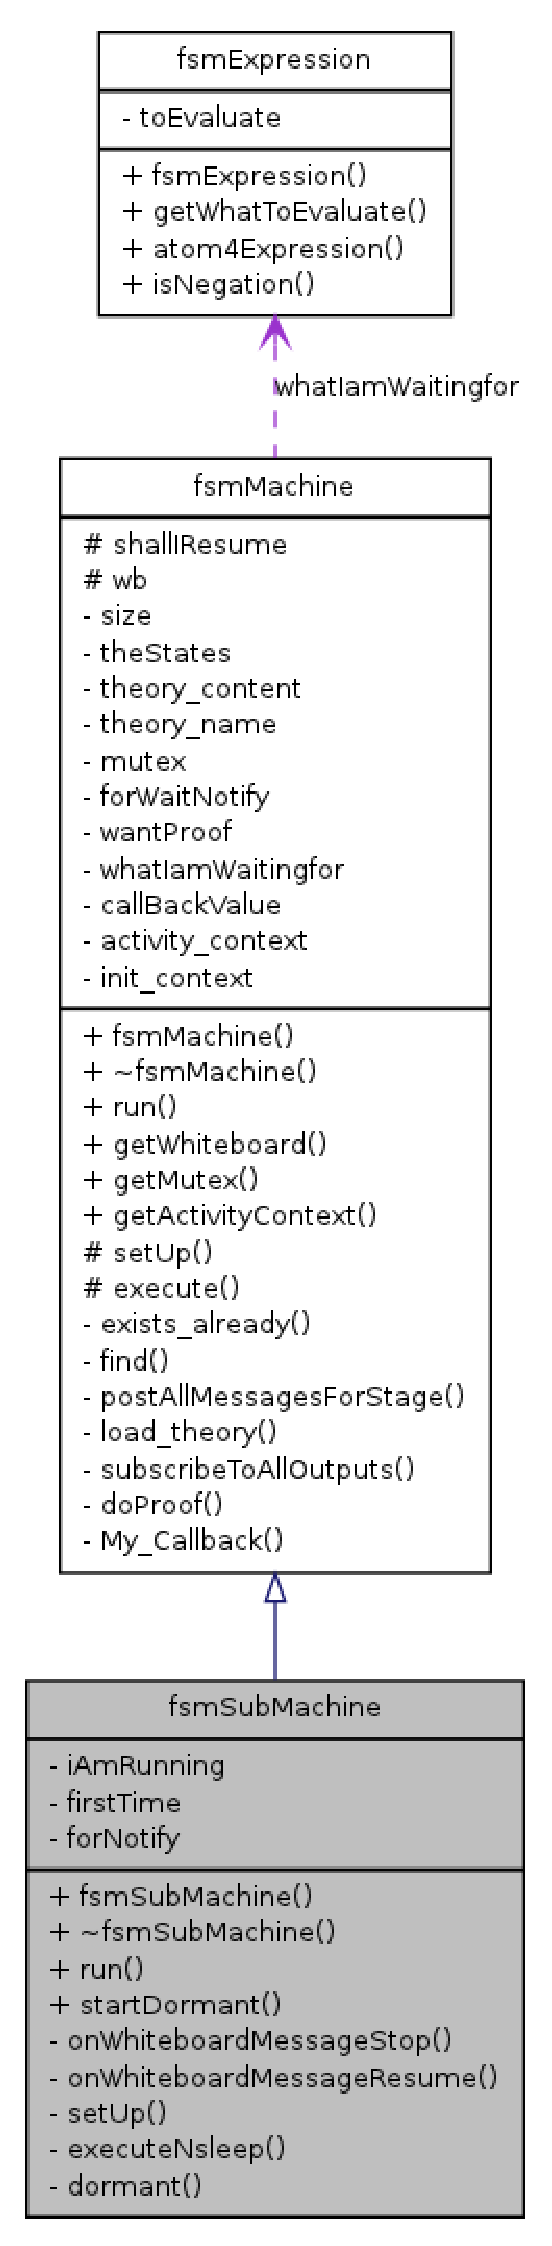
\includegraphics[height=8in]{classfsmSubMachine}
\caption{There are machines that start immediately, and a special class of sub-machines
that can in addition be started dormant, and resumed using postings on the
whiteboard}
\end{figure}

A transition has a source state, a target state and is labeled by a logic expression.
States are identified by their ID, but can have a name. They have a container
for the transitions coming out of the state.
A state's activity is a complex object holding 3 containers of postings.
They are on entry postings, on exit postings and internal postings. There
is also the possibility to invoke one C++ known function for each of these
stages.

\begin{figure}
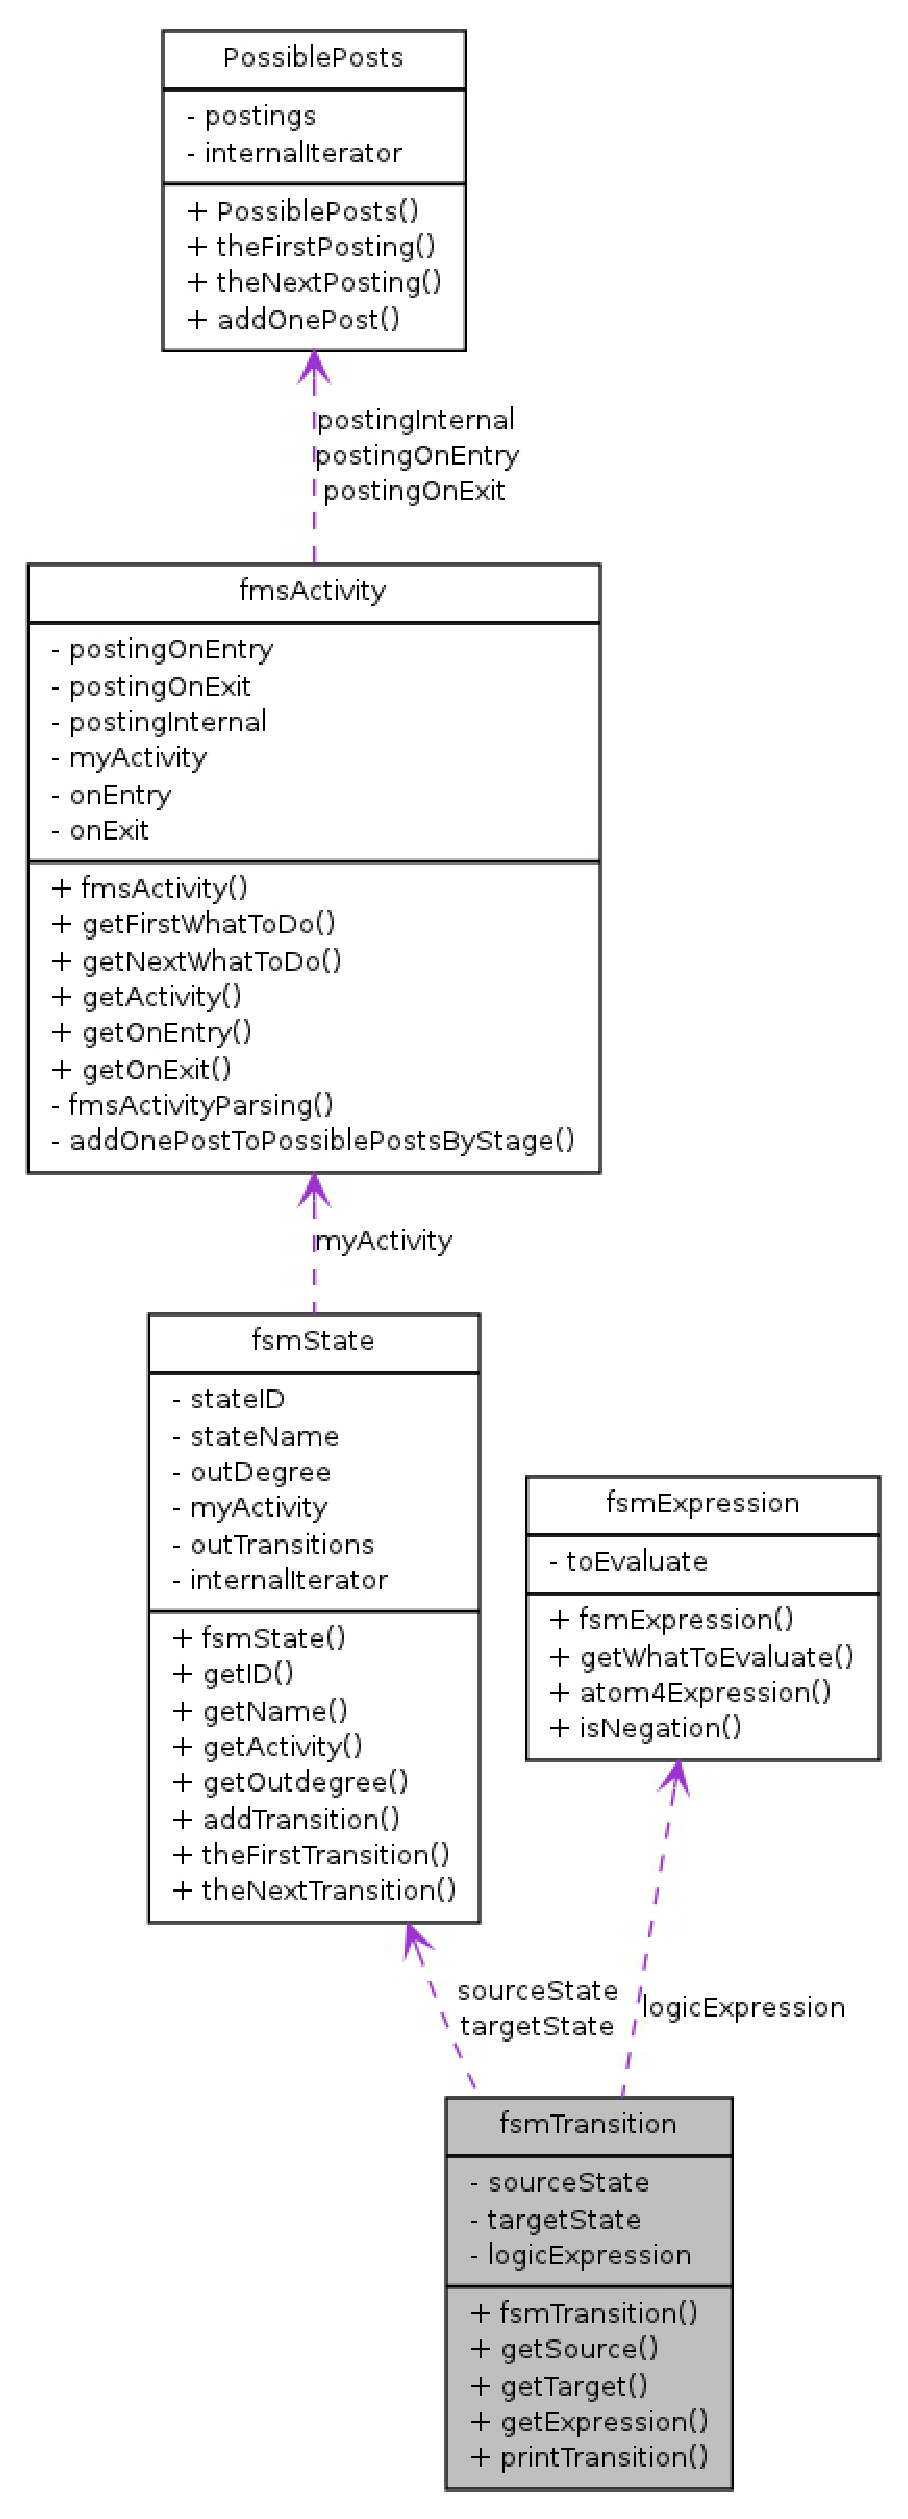
\includegraphics[height=8in]{classfsmTransition}
\caption{ Class structure in the implementaiton of FSMs ({\tt gubehaviorinterpreter})}
\end{figure}




\subsection{Transition Table}

\subsubsection{The List of Transitions}
 A Transition file starts with {\tt T} and contains
one transition for each line. This constitutes the transition table
of the finite state machine.
\begin{center}
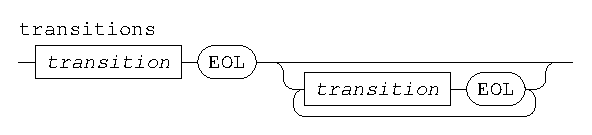
\includegraphics{transitions}
\end{center}

\subsubsection{Transitions}
 A {\tt transition} is indicted by identifying the
source state, the predicate that labels the transition and
the target state.
\begin{center}
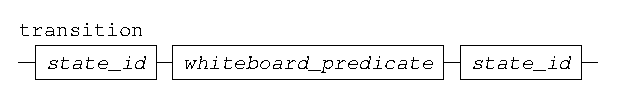
\includegraphics{transition}
\end{center}
%
\subsubsection{State Identifiers}
A {\tt state\_id} is currently only an integer.
In a future implementation, it should optionally also be a name.
\begin{center}
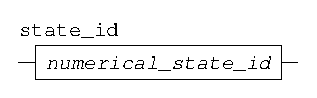
\includegraphics{state_id}
\end{center}
%
%
\subsection{The Actions in the States}
%
\subsubsection{The Actions}
 An actions file starts with {\tt A} and contains
one state description for each line. This constitutes the list of states 
of the finite state machine. The initial state is the last one listed
\begin{center}
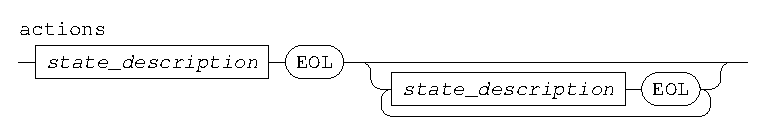
\includegraphics{actions}
\end{center}
%
\subsubsection{State Description}
 A {\tt state\_description} is 
A state id (currently a number) and a tab, followed
by an optional state name (convention is all upper case)
and a bar. It finished with a {\tt description}.
\begin{center}
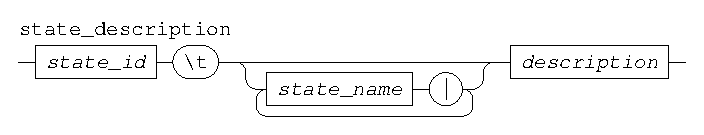
\includegraphics{state_description}
\end{center}
%
\subsubsection{Description}
A {\tt description} is intended to describe the behavior
of a state. 
 Currently , the {\tt onEntry\_part} and the
{\tt onExit\_part} will always be executed exactly once.
 The {\tt onEntry\_part}  before anything, while
the {\tt onExit\_part} after anything.
The {\tt internal\_part} will only be executed after all
exiting transitions have evaluated and not fired.
\begin{center}
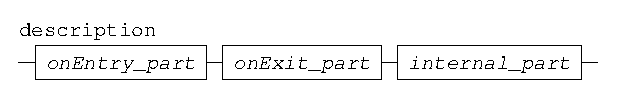
\includegraphics{description}
\end{center}
%
\subsubsection{The parts }
All parts can be empty, but the
{\tt onExit\_part} and 
the {\tt onEntry\_part} must be terminated by {\tt /}.
\begin{center}
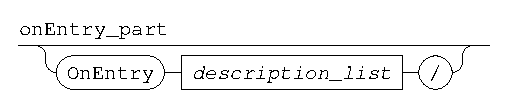
\includegraphics{onEntry_part}
\end{center}
\begin{center}
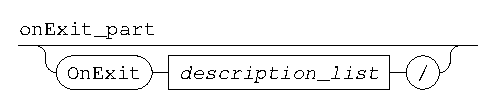
\includegraphics{onExit_part}
\end{center}
\begin{center}
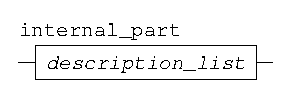
\includegraphics{internal_part}
\end{center}

%
\subsubsection{Description List}
A {\tt description\_list} could be empty. All postings
messages go before any call to a executable procedure, because for this
one there should be only one.
\begin{center}
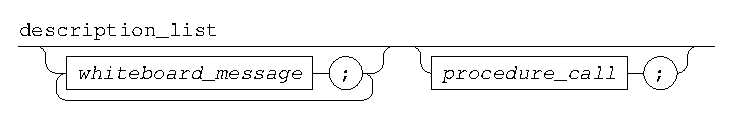
\includegraphics{description_list}
\end{center}

%
\subsubsection{Whiteboard Message}
A message will be posted to the whiteboard. The message
type is compulsory, but the content is optional; in which case
it will be considered an empty string.
\begin{center}
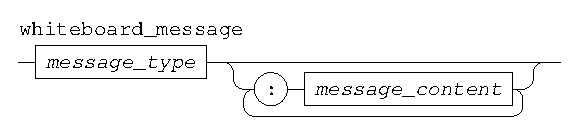
\includegraphics{whiteboard_message}
\end{center}

%
\subsubsection{Procedure Call }
A {\tt procedure\_call} is used to embed code in the finite state machine.
Currently only C++ is implemented, and the {\tt procedure\_invocation} must
be compiled with the finite state machine.
\begin{center}
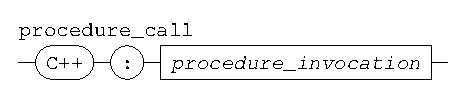
\includegraphics{procedure_call}
\end{center}
%

%
\subsubsection{Procedure Invocation }
A {\tt procedure\_invocation} is used to invoke a procedure in code in the finite state machine.
Currently only C++ is implemented, and the {\tt procedure\_name} must
be a string mapped against a procedure compiled into the finite state machine
\begin{center}
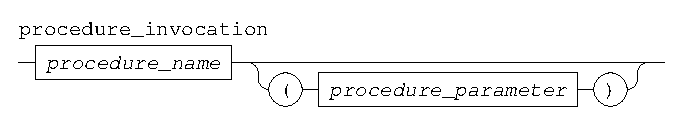
\includegraphics{procedure_invocation}
\end{center}
%

%
\subsubsection{Procedure Parameter }
A {\tt procedure\_invocation} is used to invoke a procedure in code in the finite state machine.
Currently only C++ is implemented, and the {\tt procedure\_name} must
be a string mapped against a procedure compiled into the finite state machine
\begin{center}
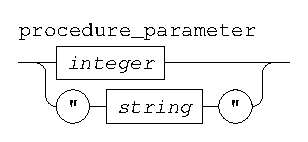
\includegraphics{procedure_parameter}
\end{center}
%
%
%






\end{document} 
